\documentclass[12pt]{article}%%contributed-IMS
\usepackage{amsthm,amsmath,amsfonts,amssymb,natbib}
\usepackage{graphicx}
\pagestyle{empty}

%\setlength{\textwidth}{7in}
%\setlength{\oddsidemargin}{-.25in}
%\setlength{\evensidemargin}{-.25in}


\newtheorem{lem}{Lemma}

\title{TBD}
\author{Nam H. Lee \& c}
\begin{document}
\maketitle

\section{Overview}
For each (undirected) pair $ij$ of $n$ vertices and each $t \in [0,1]$,
we let $N_{ij}(t)$ be the number of (undirected) communication events between vertex $i$ and vertex $j$, where each event is marked with one of the communication content topic classes $\{1,2\}$. 
Let, for each $t \in [0,1]$,
$$
\mathcal D(t) = \{ (\tau_\ell, ij_{\ell}, k_{\ell}) : \ell=1,\ldots, N(t) \},
$$ 
where $N(t) = \sum_{i<j} N_{ij}(t)$ and for simplicity, let 
$$
\mathcal D = \mathcal D(1).
$$ 

In this paper, we consider a problem of classifying the $n$ vertices into two groups after seeing $\mathcal D$, where the members of each class have the similar degrees of interests in topics from two content topic classes.  For this, we propose a classification algorithm derived from an EM-based paramter estimation procedure. 

To formulate our EM-based algorithm, we introduce a model for $\mathcal D$ through a data augmentation principle.  The hidden variables augmenting the data are the collection of random variables $\{\Lambda_{i,k}(t)\}$, where $\Lambda_{i,k}(t)$ is the degree of vertex $i$'s interest in topics from content topic class $k$ at time $t$. We assume that each $\Lambda_{i,k}(t)$ is a strictly positive random variable such that for some fixed constant $\lambda_i \in (0,\infty)$,
\begin{eqnarray}
\lambda_i = \Lambda_{i,1}(t) + \Lambda_{i,2}(t).
\end{eqnarray}
Our model, yielding the observation $\mathcal D$, is then to be a doubly stochastic marked Poisson process whose latent intensity process is specified by the $n\times 2$ random matrix
\begin{eqnarray}
\Lambda(t) = (\Lambda_{i,k}(t); i=1,\ldots,n, k=1,2).
\end{eqnarray}
For convenience, we denote the $i$-th row of $\Lambda(t)$ by $\Lambda_i(t)$. 

To demonstrate the peformance of our classification algorithm, we will also consider a so-called vertex nomination problem, in which the memembers of a particular class is already known and the objective is then to decide whether or not the class is to be expanded further and if to be expanded, which (single) vertex is to be included next. A solution to the vertex nomination problem is likely to be useful if some other information other than $\mathcal D$ is available.  On the other hand, we will also denomstrate the peformance of our classification algorithm when the only available information is $\mathcal D$ and the vertex nomination is then interpreted as a two-pass procedure.  

\section{Single-period model}
For each vertex $i$ and time $t\in[0,1]$, let 
\begin{eqnarray}
X_i(t) = (X_{i,1}(t), X_{i,2}(t)),
\end{eqnarray}
where
\begin{eqnarray}
X_{i,k}(t) = \frac{\Lambda_{i,k}(t)}{\Lambda_i(t)},
\end{eqnarray}
and note that each $X_i(t)$ is a probability vector. 

For each (undirected) pair $ij$, we assume that 
the process $N_{ij} = (N_{ij}(t):t\in[0,1])$ is   
a doubly stocastic Poisson process that whose intensity process is  
\begin{eqnarray}
\Lambda_{ij}(t) = \lambda_i \lambda_j (X_{i,1}(t)X_{j,1}(t) + X_{i,2}(t)X_{j,2}(t)).
\end{eqnarray}
A particularly useful chracterization is to describe each $N_{ij}$ as a process obtained 
by thinning a homogeneous Poisson process $C_{ij}$ whose constant intensity is $\lambda_i \lambda_j$.  
This affords an interpretation that each $t$ such that $C_{ij}(t) = C_{ij}(t-) +1$ 
is a potential communication opportunity between vertex $i$ and vertex $j$, 
and at each such $t$, depending on values of $X_i(t)$ and $X_j(t)$, 
the opportunity may or may not give rise to an actual communication event, i.e.\ $t$ such that $N_{ij}(t) = N_{ij}(t-) +1$. To be more precise, it is our assumption that given the filtration 
$$
\mathcal F_{ij}^\Lambda(t) = \sigma(\Lambda_i(s), \Lambda_j(t): s \le t), 
$$
if $C_{ij}(t) = C_{ij}(t-)+1$, then
$N_{ij}(t) = N_{ij}(t-) + 1$ with probability $\Lambda_{ij}(t)$ and the topic mark is of content class $k$ with probaiblity 
$$
\frac{X_{i,k}(t)X_{j,k}(t)}{X_{i,1}(t)X_{j,1}(t) + X_{i,2}(t)X_{j,2}(t)}
=
\frac{\Lambda_{i,k}(t)\Lambda_{j,k}(t)}{\Lambda_{i,1}(t)\Lambda_{j,1}(t) + \Lambda_{i,2}(t)\Lambda_{j,2}(t)}.
$$
Now, we fix a stationary diffusion process $Y_i=(Y_i(t):t\in [0,1])$ such that  
\begin{eqnarray}
dY_i(t) = \mu(Y_t(t)) dt + \sigma_i(Y_i(t)) dB_i(t),
\end{eqnarray}
where each $\mu_i$ and $\sigma_i$ are twice continuously and boundedly differentiable functions, and $B_1,\ldots,B_n$ are independent standard Brownian motions.
In fact, in this paper, for concreteness, we assume that 
\begin{eqnarray}
dY_i(t) = \beta_i (\mu_i - Y_i(t)) dt + \sigma_i dB_i(t),
\end{eqnarray}
for some fixed constants $\mu_1,\ldots, \mu_n \in \mathbb R$, and $\sigma_1 = \ldots = \sigma_n \in (0,\infty)$ and $\beta_1 = \ldots = \beta_n \in (0,\infty)$. 
Then, we assume that 
\begin{eqnarray}
X_{i,1}(t) = \frac{1}{1+\exp(-Y_i(t))}.
\end{eqnarray}
For future reference, we let
\begin{eqnarray}
&\mu = (\mu_1,\ldots, \mu_n),\\
&\beta = (\beta_1,\ldots,\beta_n),\\
&\sigma = (\sigma_1,\ldots,\sigma_n),\\
&\lambda = (\lambda_1,\ldots,\lambda_n),\\
&\psi = (\mu,\beta,\sigma,\lambda).
\end{eqnarray}
The term single period here emphasises the fact that the parameter $\psi$ 
are assumed to be constant within time period $[0,1]$. 

\section{Estimation by EM procedure}
\subsection{Preliminaries}
Let
\begin{enumerate}
\item[(i)] $M_{ij}$ is the (total) number of messages between vertex $i$ and vertex $j$,
\item[(ii)] $\tau_{ij}(\ell)$ is the time at which occurred the $\ell$-th communication event  between vertex $i$ and vertex $j$.
\end{enumerate}
The EM algorithm is then given the $r$-th estimate $\psi^r$, find the $(r+1)$-st estimate $\psi^{r+1}$ by 
finding $\psi$ that maximizes the expected value of the following random variable:
\begin{eqnarray}
F^r(\psi):=\prod_{i<j} f_{ij}(\mathcal D_{ij});X_i^r,X_j^r,\psi) \prod_{i=1}^n f_{i}(Y_i^r;\psi),
\end{eqnarray}
where 
\begin{enumerate}
\item[(i)] $Y_i^r$ is a diffusion process whose distribution is a conditional distribution of $Y_i$ given the observation $\mathcal D$ with the unconditional distribution of $Y_i$ for the $r$-th estimated parameter $\psi^r$,
\item[(ii)] $f_{i}(\cdot;\psi)$ is the likelihood of the $i$-th vertex 
process' sample path $Y_i$ with the parameter $\psi$,
\item[(iii)] $f_{ij}(\cdot;X_i^r,X_j^r,\psi)$ specifies the conditional likelidhood given $X_i^r,X_j^r$ of 
observing message at time 
$$
\tau_{ij}(1),\ldots, \tau_{ij}(M_{ij}),
$$
repsectively, about topic 
$$
\kappa_{ij}(1),\ldots, \kappa_{ij}(M_{ij}).
$$
\end{enumerate}
It can be seen that
\begin{eqnarray*}
L_{ij}^r(\psi) 
&:= & \log f_{ij}(\mathcal D_{ij} ;X_i^r,X_j^r,\psi) \\
&= &  \sum_{i<j} 
\left(
\sum_{\ell=1}^{M_{ij}} \log(\lambda_i) + \log(\lambda_j) + 
\log(X_{i,\kappa_{ij}}(\tau_{ij}(\ell))) +
\log(X_{j,\kappa_{ij}}(\tau_{ij}(\ell))) \right) \\
&\ &  - \sum_{i<j} \lambda_i\lambda_j \int_0^1 X_{i,1}^r(s)X_{j,1}^r(s)+X_{i,2}^r(s)X_{j,2}^r(s) ds,
\end{eqnarray*}
and that 
\begin{eqnarray*}
R_i^r(\psi) 
&:= & \log (f_i(Y_{i}^r(t);\psi))\\
&= &
\left. \frac{\beta_i}{\sigma_i^2} \left( \mu_i Y_t^r - \frac{1}{2} (Y_t^r)^2\right) \right|_0^1
- \frac{1}{2} \frac{\beta_i^2}{\sigma_i^2} \int_0^1 (\mu_i-Y_{i}^r(t))^2 dt + \frac{\beta_i}{2}. 
\end{eqnarray*}
Then, we have 
\begin{eqnarray}
Q^r(\psi) = \log(F^r(\psi)) := \sum_{i<j} L_{i,j}^r(\psi) + \sum_{j} R_j^r(\psi).  
\end{eqnarray}

While we give the details for our $M$-step and then our $E$-step in the next two sections, 
we list here some facts relevant in their derivation:
\begin{description}
\item[(i)] Each random variable $L_{ij}^r(\psi)$ is parameterized only by $\lambda_i$ and $\lambda_j$, 
\item[(ii)] Each random variable $R_{i}^r(\psi)$ is parameterized only by the $\mu_i, \beta_i$ and $\sigma_i$,
\item[(iii)] While unconditionally, the diffusion processes $Y_1,\ldots, Y_n$ are independent,
conditionally on $\mathcal D$, $Y_1,\ldots,Y_n$ need not be independent.
\end{description}

\subsection{EM-steps}
In this section, we specifies our EM steps, yielding a sequence of estimates:
\begin{eqnarray}
\{\psi^r: r \in \mathbb N\}.
\end{eqnarray}
Let
\begin{eqnarray}
\Lambda_{(\ell,+)}^r(s)
=
\lambda_{(\ell)}^r \lambda_{(\ell)}^r X_{i(\ell),k(\ell)}^r(s)X_{j(\ell),k(\ell)}^r(s),
\end{eqnarray}
and then, 
\begin{eqnarray}
\Lambda_{(\ell,-)}^r(s)
=
\lambda_{(\ell)}^r \lambda_{(\ell)}^r (1-X_{i(\ell),k(\ell)}^r(s))(1-X_{j(\ell),k(\ell)}^r(s)).
\end{eqnarray}
Let 
\begin{eqnarray}
W_\ell = \Lambda_{(\ell,+)}(\tau_\ell) \exp\left(-\int_{\tau_{(\ell-1}}^{\tau(\ell)} \sum_{i<j} \Lambda_{i,j}^r(s) ds\right),  
\end{eqnarray}
Then, let 
\begin{eqnarray}
W = \prod_{\ell=1}^M W_{\ell}.
\end{eqnarray}
For simplicity, we let $\langle \cdot \rangle$ be the inner-product operator, i.e.\ for $x,y\in\mathbb R^d$, $\langle x, y \rangle = \sum_{\ell=1}^d x_i y_i$.   

\begin{eqnarray}
W^r = \prod_{\ell=1}^{M} \exp\left(-\int_{\tau_{\ell-1}}^{\tau_\ell} \Lambda^r(s) ds\right)
\end{eqnarray}

Our main results in this section are the specification of our EM steps.  Let $\psi^r$ denote the $r$-th estimate from our $EM$-sequence, and for each $\psi \in \Psi$, define  
\begin{eqnarray}
Q_r(\psi) = \mathbf E_*[F^r(\psi)],
\end{eqnarray}
where $\mathbf E_*$ denote the expectation operator conditioal on the data $\mathcal D$.  
The E-step can be completed using the following lemma:
\begin{lem}
Let $\xi$ be an $\mathcal F^r$-measurable random variable, where
\begin{eqnarray}
\mathcal F^r = \sigma(Y_s^r: s \le t).
\end{eqnarray}  
Then, 
\begin{eqnarray}
\mathbf E_*[\xi] = \mathbf E[\xi W^r]/\mathbf E[W^r].
\end{eqnarray}
\end{lem}
Now, the M-step can be dervied explicited.  That is, the $(r+1)$-st estimate $\psi^{(r+1)}$ satisfies the following equations:
\begin{eqnarray*}
\sigma_{i,r}^2 &=& 2 \mathbf E_*\left[ \beta_i \int_0^1 \left(\mu_i - Y_i^r(t)\right)^2dt 
- \left(\left.\mu_i Y_i^r(t) - \frac{1}{2} (Y_i^r(t))^2\right)\right|_0^1\right]\\\mu_{i,r} 
&=&  \frac{\left. \mathbf E_*[Y_i^r(t)^2]\right|_0^1}{\left.\mathbf E_*[Y_i^r(t)\right|_0^1}\\ 
&\ &\pm
\sqrt{
\left(\frac{\left.\mathbf E_*[Y_i^r(t)^2]\right|_0^1}{\left.\mathbf E_*[Y_i^r(t)]\right|_0^1}\right)^2 
-
4\left( \frac{\left.\mathbf E_*[Y_i^r(t)^2]\right|_0^1}{\left.\mathbf E_*[Y_i^r(t)]\right|_0^1} \int_0^1\mathbf E_*[Y_i^r(t)]dt - \int_0^1 \mathbf E_*[Y_i(t)^2] dt\right)}\\
\beta_{i,r}
&=&
\frac{\left. \mathbf E_*[Y_i^r(t)] \right|_0^1}{\mu_{i,r} - \int_0^1 \mathbf E_*[Y_i^r(t)]dt}\\
\lambda_{i,r} 
&=& 
\frac{M_i}
{
\sum_{j\neq i} \lambda_j \int_0^1 \mathbf E_*[\langle X_i^r(s), X_j^r(s)\rangle] ds.
} 
\end{eqnarray*}


\section{Test of goodness of fit via Kalman-Bucy filtering}
Our model for the communication records is a so-called multichannel doubly stochastic Poisson process 
which is comprised of $n(n-1)/2$ single-channel doubly stochastic Poisson process $\{N_{ij}(t):t\in[0,1]\}$ 
that are conditionally mutually independent Poisson process given the information process, 
which is our $X=(X_1,\ldots,X_n)$.  In particular, each $\{N_t^{(i,j)} : t \in [0,1]\}$ is a doubly stochastic 
Poisson process with corresponding intensity process whose intensity process is $\Lambda_{ij}(\cdot)$.  

Consider estimating the intensities at time $t$ in terms of an observed counting path on the interval $[0,t]$,
with the estimator being linear.  That is, the estimate $\Lambda_{ij}^{*}(t)$ of $\Lambda_{ij}(t)$ is to be of 
the form:
\begin{eqnarray}
\Lambda_{ij}^{*}(t) = a_{ij}(t) + \int_0^t h_{ij}(t,u) dN_{ij}(u),
\end{eqnarray}
for some deterministic function $a_{ij}(t)$ and impulse response function $h(t,u)$.  

It follows from the theory [Donald Snyder, Thm 6.5.1] that the corresponding the minimum mean squared error estimate
denoted by $\widehat{\Lambda}_{ij}(t)$ is the following:
\begin{eqnarray}
\widehat{\Lambda}_{ij}(t) = \mathbf E[\Lambda_{ij}(t)] + \int_0^t h_{ij}(t,u)\left[dN_{ij}(u) - E(\Lambda_{ij}(t))du\right],
\end{eqnarray}
where the optimum impulse response $h_0(t,u)$ is the solution to the integral equation:
\begin{eqnarray}
h_{ij}(t,u) E(\Lambda_{ij}(u)) 
+
\int_0^t h_{ij}(t,s) C_{\Lambda_{ij}}(s,u) ds = C_{\Lambda_{ij}}(t,u)
\end{eqnarray}
for $0 \le u \le T$.  Here, $C_{\Lambda_{ij}}$ is the covariance function of the intensity process.  Furthermore,
the result minimum mean-square error is given by:
\begin{eqnarray}
\mathbf E[(\Lambda_{ij}(t) - \widehat{\Lambda}_{ij}(t))^2] = h_{ij}(t,t) \mathbf E[\Lambda_{ij}(t)]. 
\end{eqnarray}
In fact, from its relation to a linear filtering problem 
for observations that contains additive noise, the Kalman-Bucy algorithm satisfies
the folowing set of equations:
\begin{eqnarray}
d\widehat{X}_{ij}(t)  = 
\end{eqnarray}

\begin{eqnarray}
dX_i^*(t) = 
\beta_i (\mu_i - X_i^*(t)) dt  
+
\Sigma_{t} () \texttt{diag}^{-1}[\lambda_k^k(X_t^*) [dN_t - \lambda_t(X_t^*)dt].
\end{eqnarray}
We can take
\begin{eqnarray}
\widehat{\lambda}_{ij}(t) 
&=& \mathbf E\left[ \lambda_{ij}(t) \left| \mathcal F^{N}_t\right.\right] \\
&=& \mathbf E\left[ \lambda_{ij}(t) D(t)\right]/\mathbf E\left[D(t)\right]
\end{eqnarray}
\begin{figure}
\begin{center}
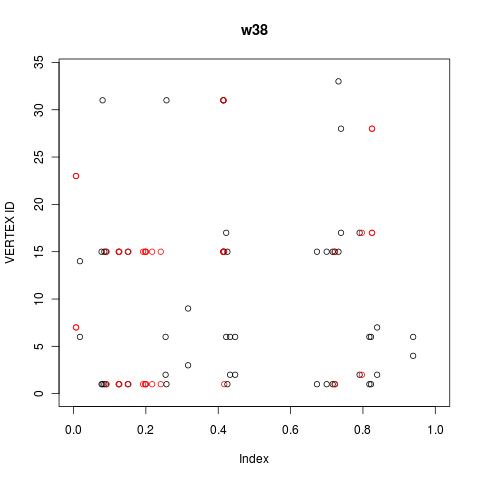
\includegraphics[scale=0.30]{v34_myDdata_w38.png}
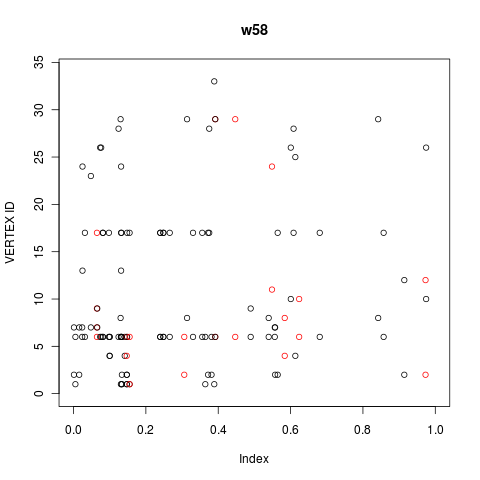
\includegraphics[scale=0.30]{v34_myDdata_w58.png}
\end{center}
\caption{w38 versus w58, the $\mathcal D(V_{34})$ data, where $V_{34} =\{1,2,\ldots, 34\}$}
\label{theDplot}
\end{figure}

\begin{figure}
\begin{center}
{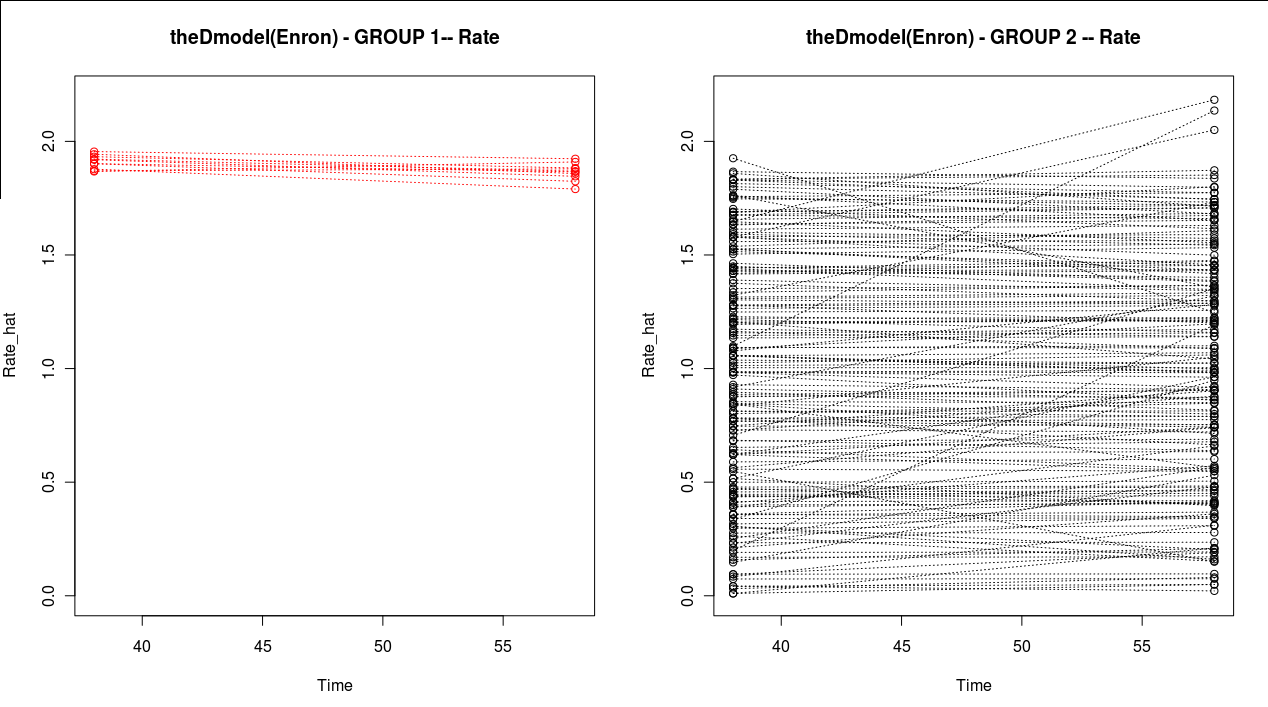
\includegraphics[scale=0.20]{v184_w38vsw58_Rate.png}}
{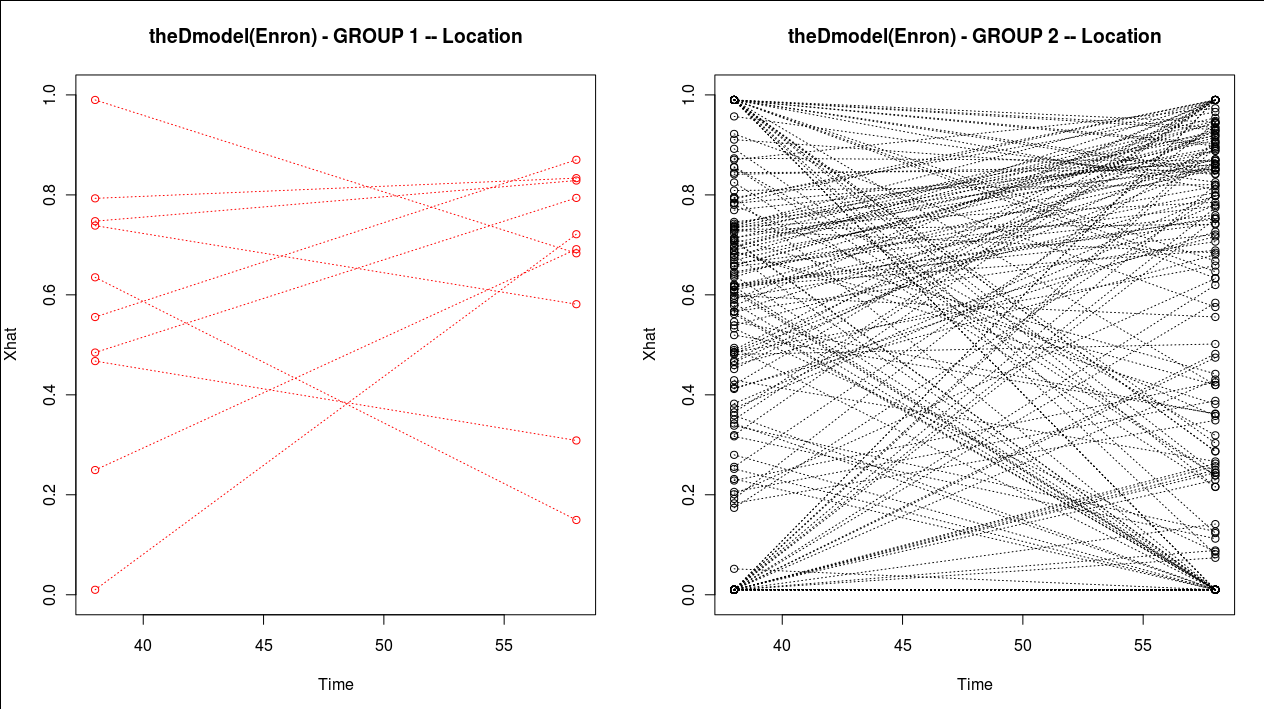
\includegraphics[scale=0.20]{v184_w38vsw58_Location.png}}
\end{center}
\caption{w38 versus w58, $\hat{\lambda}_i$ and $\hat{\mu}_i$ obtained by the initialization step of the EM alglorithm on $\mathcal D = \mathcal D(V_{184})$, where $V_{184} = \{1,\ldots, 184\}$}
\label{cepplot}
\end{figure}

\section{Greedy algorithm for iterative vertex nomination}
Our main result of this paper concerns an algorithm 
for correctly assigning each vertex into one of two classes, where witnin each group, all the members  
have the same parameter i.e.\ if vertex $i$ and vertex $j$ are in the same
class, then $\psi_i = \psi_j$.  
In this section, we provide a greedy algorithm for arriving at a partition 
of the vertex set which is likely to be the true partition of 
the vertex set that  have produced the data $\mathcal D$.

For the initial step $q=1$, suppose that we have 
an arbitrary partition $(C_1(1), C_2(1))$ of $\{1,\ldots, n\}$. 
Let $\psi^1$ be the output of our EM algorithm, where we assume that within each group,
all vertice have the same paramter.  Then, for each pair $i, j \in C_k(1)$, $\psi_i^1 = \psi_j^1$.  
Let
\begin{eqnarray}
Q(1) : = \mathbf E_{\psi(1)}\left[\log(f(\mathcal D, Y;\psi^1))\right],
\end{eqnarray}
where $f(;\psi)$ denote the likelikehood function of observing $\mathcal D$ and $Y$ with the given parameter $\psi$ (see the next section for more details about this). 
Next, for the $(r+1)$-st iteration, suppose that we have a partition $(C_1(r), C_2(r))$ from the $r$-th iteration. 
If $C_2(r) = \varnothing$, then our partitioning algorithm terminates, yielding the $r$-th partition 
$(C_1(r), C_2(r))$ as the final output.  So, we assume that $C_2(r)\neq \varnothing$.  Then, for some $\ell > 0$ and $m > 0$ with $\ell + m = n$, we have 
\begin{eqnarray}
&C_1(r) = \{u_1,\ldots, u_\ell\},\\
&C_2(r) = \{v_1,\ldots, v_m\}.
\end{eqnarray} 
For each $i \in C_2(r)$, let 
\begin{eqnarray}
&C_1^{i}(r) = C_1(r) \cup \{i\}, \\
&C_2^{i}(r) = C_2(r) \setminus \{i\}.
\end{eqnarray}
Now, for each $i$, let $\psi^{i,r}$ be the EM estimate of $\psi$ with the partition $(C_1^{i}(r), C_2^{i}(r))$, and let 
\begin{eqnarray}
Q^{i}(r) = \mathbf E_{\psi^{i,r}}\left[\log(f(\mathcal D,Y;\psi^{i,r}))\right].
\end{eqnarray}
If for all $i \in C_2(r)$, $Q^{i}(r) \le Q(r)$, then the algorithm terminates, yielding 
$(C_1(r), C_2(r))$ as the final partitioning.  Otherwise, we set 
\begin{eqnarray}
i^* = \arg\max_{i \in C_2(r)} Q^{i}(r),
\end{eqnarray}
and let 
\begin{eqnarray}
&C_1(r+1) = C_1(r) \cup \{i^*\},\\
&C_2(r+1) = C_2(r) \setminus \{i^*\}.
\end{eqnarray}

\section{Experiment Results}
In this section, we present the experiment results done on the so-called Enron E-mail data using the algorithms 
presented in this paper.  The raw full Enron E-mail data does not necessarily conform to our $\mathcal D$ data 
format as we presented in this paper.  For example, some E-mails contain more than one receiver or in some cases, 
the sender and the receiver are one and the same.  Unfortunately, there is not a conventionally accepted method for 
assigning an E-Mail to one or two categories that everyone can agree on, and apriori, our model is not adequate to
handle such data.  While we hope to extend our algorithm that can handle the full data set in near future, in this
paper, we procede to apply our algorithms to a data set that is derived from the raw full Enron Email data so that 
it fits the format of $\mathcal D$.  One way to achieve this is to consider only the messages such that 
the receiver is exactly one that is also different from the sender and also if there is any message with 
the same time stampe even after that, we randomly perturb the time stamp minutely ad hoc so that the resulting data conform
to our framework.  We consider two sets of data.  Each one for approximately four months periods starting at the week of 38 and the week of 58 since Jan 1, 1970.  These weeks are of interest in this paper because there are other studies done on the Enron Email data that suggests that the first data set is significantly different from the second in their communication pattern (cf.\ the importance sampling method in [GC]).  The method in [GC] relies on a graph theoretic statistic 
and also suggests that the ten vertices out of 184 vertices form a coherent social/communication group.   
We aim to support the same claim here instead using our classification algorithm.  

The subset of the data $\mathcal D$ is presented above only for thirty four vertices in the data, but our experiment is done for 184 vertices.  For clarity, for each sub-collection $\mathcal V$ of vertices, 
we let $\mathcal D(V)$ denote the subsubet of $\mathcal D$, where both the sender and the receiver are from $\mathcal V$. The figure in Figure \ref{theDplot} is for $\mathcal D(V) \subset \mathcal D$, where $V = \{1,\ldots,34\}$.  In  Figures \ref{cepplot}, the left hand side is for week 38 and the right hand side is for week 58.


The algorihm run on a simulated data shows that it does right thing.  
\begin{figure}
\begin{center}
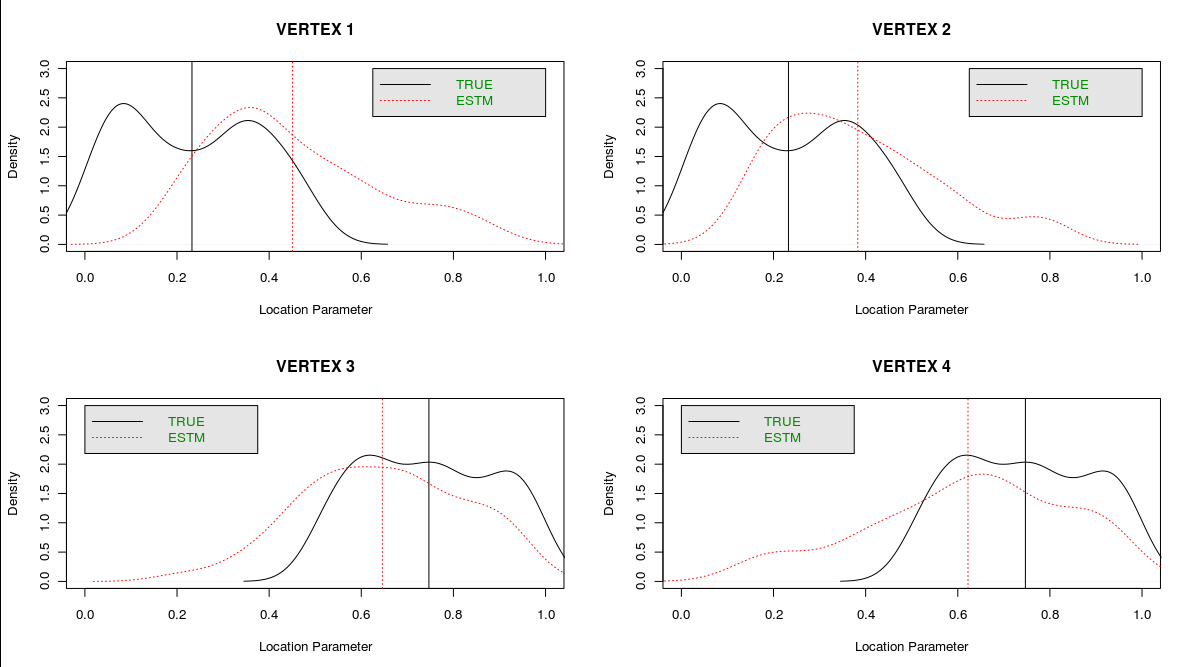
\includegraphics[scale=0.30]{comparing_density.png}
\end{center}
\caption{Performance of the algorithm on simulated data}
\end{figure}



\end{document}
